\documentclass[11pt]{article}
\usepackage[T1]{fontenc}
\usepackage[utf8]{inputenc}
\usepackage{lmodern}
\usepackage[margin=1in]{geometry}
\usepackage{amsmath,amssymb,amsthm,mathtools}
\usepackage{enumitem,booktabs,microtype}
\usepackage{tikz}
\usetikzlibrary{arrows.meta,positioning,calc,patterns,fit}
\usepackage[hidelinks]{hyperref}
\hypersetup{pdftitle={Spectral scalar curvature and uniform Urysohn width},
  pdfauthor={OpenAI},pdfsubject={A spectral extension of uniform scalar-curvature width bounds}}
\newtheorem{theorem}{Theorem}[section]
\newtheorem{lemma}[theorem]{Lemma}
\newtheorem{proposition}[theorem]{Proposition}
\newtheorem{corollary}[theorem]{Corollary}
\theoremstyle{definition}
\newtheorem{definition}[theorem]{Definition}
\theoremstyle{remark}
\newtheorem{remark}[theorem]{Remark}
\newcommand{\R}{\mathbb R}
\newcommand{\dd}{\mathrm d}
\newcommand{\vol}{\mathrm{vol}}
\newcommand{\Dcal}{\mathcal D}
\DeclareMathOperator{\Scal}{Scal}
\DeclareMathOperator{\Ric}{Ric}
\DeclareMathOperator{\Hess}{Hess}
\DeclareMathOperator{\tr}{tr}
\DeclareMathOperator{\diver}{div}
\DeclareMathOperator{\dist}{dist}
\DeclareMathOperator{\diam}{diam}
\DeclareMathOperator{\supp}{supp}
\DeclareMathOperator{\UW}{UW}
\numberwithin{equation}{section}
\setlength{\emergencystretch}{1.5em}
\setcounter{tocdepth}{1}
\title{Spectral scalar curvature\protect\\and uniform Urysohn width}
\author{OpenAI}
\date{October 5, 2026}
\begin{document}
\maketitle
\begin{abstract}
For every $n\ge4$, a complete connected smooth Riemannian $n$-manifold
without boundary satisfying $-4\Delta+\Scal\ge1$ as a quadratic-form
inequality admits a continuous map to a simplicial complex of dimension
at most $n-2$ whose entire fibers have diameter bounded only in terms
of $n$. The bound is measured in the original metric. This extends the
uniform Urysohn width theorem from a pointwise scalar-curvature lower
bound to a spectral lower bound.
\end{abstract}
\tableofcontents
\clearpage
\section{Introduction}\label{sec:intro}

Positive scalar curvature is expected to force a manifold to lose two
dimensions at a controlled geometric scale. A spectral lower bound
mixes scalar curvature with the energy of a test function and permits
negative scalar curvature on parts of the manifold. We show that the
uniform width conclusion survives this weakening. The geometric input
is the stabilized width theorem of \cite{OpenAIWidth}, stated precisely
in Theorem~\ref{interface:width}; the work here constructs its hypotheses
from the spectral inequality.

Let $(M^n,g)$ be a connected complete smooth Riemannian manifold without
boundary. We use $\Delta_g=\diver_g\nabla_g$ and integrate against the
Riemannian volume density. The \emph{normalized spectral scalar-curvature
bound} is
\begin{equation}\label{eq:spectral-bound}
 \int_M\bigl(4|\nabla_g\phi|_g^2+\Scal_g\phi^2\bigr)\,\dd\vol_g
 \ge \int_M\phi^2\,\dd\vol_g
 \qquad\bigl(\phi\in C_c^\infty(M;\R)\bigr).
\end{equation}
Thus $-4\Delta_g+\Scal_g\ge1$ in the quadratic-form sense. This is
the definition on noncompact manifolds as well; it does not require
a lowest eigenvalue to be attained.

For a metric space $X$ and an integer $d\ge0$, its \emph{Urysohn
$d$-width} is
\[
 \UW_d(X)=\inf_{f:X\to K}\ \sup_{y\in K}\diam_X f^{-1}(y),
\]
where $f$ is continuous and $K$ is a simplicial complex of dimension
at most $d$ with its usual polyhedral topology. The diameter refers
to the entire fiber, including all its components; empty fibers may
be omitted.

\begin{theorem}\label{thm:main}
For every integer $n\ge4$ there is a finite constant $C_n$ with the
following property. Every connected complete smooth Riemannian
$n$-manifold $(M,g)$ without boundary satisfying
\eqref{eq:spectral-bound} admits a continuous map $f:M\to K$ to a
simplicial complex of dimension at most $n-2$ such that
\[
 \diam_g f^{-1}(y)\le C_n\qquad(y\in K).
\]
In particular, $\UW_{n-2}(M,g)\le C_n$.
\end{theorem}

The constant depends only on the dimension. The theorem applies to
compact and noncompact manifolds, without orientability, spin, or
bounded-geometry assumptions. If the right side of
\eqref{eq:spectral-bound} is multiplied by $\lambda>0$, scaling the
metric to $\lambda g$ gives the fiber bound $C_n/\sqrt\lambda$.

\subsection{History and relation to earlier work}

Gromov's macroscopic dimension program relates positive scalar curvature
to the dimension of a space seen at large scales. The quantitative
formulation asks whether a fixed positive scalar-curvature normalization
forces a dimension-dependent bound for the fibers of a map to an
$(n-2)$-dimensional polyhedron. This formulation goes back to
\cite[\S\,2.A(c)]{Gromov1986}; see also
\cite[\S\,$2\frac12$]{Gromov1996} and
\cite{Gromov2023}. Uniform width is stronger than merely
asking for a finite fiber bound for each individual metric. The
stabilized partition theorem used here is the geometric input from
\cite{OpenAIWidth} that gives the uniform conclusion.

Several earlier results illustrate the distinction between the
geometric and topological versions of the problem. Early
three-dimensional distance-level diameter estimates of
Gromov--Lawson~\cite{GromovLawson1983} use vanishing rational first
homology, as clarified in Gromov's later account~\cite{Gromov2023}.
That account also gives a uniform Urysohn $1$-width bound for arbitrary
complete three-manifolds with scalar curvature bounded below by a
positive constant. Under such a uniform lower bound,
Liokumovich--Maximo~\cite{LiokumovichMaximo2023} and
Liokumovich--Wang~\cite{LiokumovichWang2026} construct Morse functions
with simultaneous area and diameter bounds on connected level
components, in the closed and complete noncompact cases, respectively.
In dimensions four and five,
Chodosh--Li--Liokumovich proved finite Urysohn $1$-width for universal
covers of closed positive-scalar-curvature manifolds under the
respective assumptions $\pi_2=0$ and $\pi_2=\pi_3=0$
\cite[Theorem~4]{ChodoshLiLiokumovich2023}. That conclusion is
qualitative and uses the topology of a compact quotient. The setting
of Theorem~\ref{thm:main} instead allows arbitrary complete manifolds
and asks for one constant depending only on the dimension.

The coefficient $4$ in \eqref{eq:spectral-bound} is natural in weighted
scalar curvature. On closed manifolds, Perelman's $\mathcal F$-functional and its lowest
eigenvalue formulation involve $-4\Delta+\Scal$, together with the
expression $\Scal+2\Delta t-|\dd t|^2$
\cite[\S\S1--2]{Perelman2002}. Gromov's torus-stabilized scalar
curvature makes the same connection through diagonal warped products
\cite[\S\S1.A--1.B]{Gromov2024}. Spectral curvature bounds also enter
the band and cube inequalities of Hirsch--Kazaras--Khuri--Zhang
\cite{HirschKazarasKhuriZhang2024}, whose hypotheses depend on the
dimension, topology, and coefficient of the scalar-curvature term.
Those inequalities control separations of boundary sets, rather than
the fibers of a map on an arbitrary complete manifold.

Our starting point is the partition theorem in
\cite{OpenAIWidth}, including its locally finite stabilized input.
The spectral-to-positive-solution passage and the warped-product
formula are established tools. The additional work is to create a
quadratic reserve from an unrestricted logarithmic drift and to adapt
the local stretching argument to a signed drift. These constructions
retain the original metric as the metric in which the final fibers
are measured. In particular, no control of a conformal factor or of
the weight at infinity is needed.

\subsection{The new constructions and the proof}

The spectral hypothesis supplies a positive smooth function $v$ with
$-4\Delta_g v+\Scal_gv\ge v$. For a metric $h$ and a smooth real
function $t$, write
\begin{equation}\label{eq:drift-scalar}
 \Dcal(h,t)=\Scal_h+2\Delta_h t-|\dd t|_h^2.
\end{equation}
Then $w=-2\log v$ satisfies $\Dcal(g,w)\ge1$.
This identity produces a weighted curvature bound, but gives no
control on the value or oscillation of $w$. The stretching construction
needs an additional reserve that grows quadratically with its drift.

The first new ingredient supplies that reserve without estimating $w$.
For an arbitrary complete metric $h$ and smooth $w$, we construct a
smooth function $u$, a global graph metric $h^+=h+\dd u^2$, and a new signed drift $t^+$ such
that
\[
 \Dcal(h^+,t^+)\ge\Dcal(h,w)+(t^+)^2-C(n).
\]
Here $C(n)$ is independent of the geometry and of $w$. The graph
equation has pressure proportional to the discrepancy $u-w$; subtracting
the graph height in the drift update turns that discrepancy into the
required square. Local barriers and an angle estimate give a global
solution even when $w$ and the geometry are unbounded at infinity.
The precise statement and proof are in Proposition~\ref{pre:reserve}.

The second ingredient stretches selected pairs of sets by increasing
the metric on a compact neighborhood. Its pressure depends on a
possibly negative drift. For a dimension-dependent $T$, the reserve
is $V(t)=t^2+T^2$. When the drift increases from $t$ to $t'\ge t$,
the local estimate retains the positive part of
$V(t')-V(t)$, because increasing a signed drift need not increase
$V$. Its loss is paid by a decrease of $\tr_h h_0$, where $h_0$ is
fixed during one round of stretching, together with an arbitrarily
small summable error. The inverse construction of the pressure is
given in Proposition~\ref{pressure:law}, and the resulting geometric estimate
is Lemma~\ref{stretch:local}.

To assemble these tools, choose a radius $D$ depending only on $n$
and maximal $D$-separated centers $x_i$ in the original metric.
Their closed radius-$D$ balls cover $M$, and their closed radius-$2D$
balls are locally finite. The local lemma is applied in rounds until
each inner ball is as far as prescribed from the exterior of its
outer ball. The trace decreases
telescope within each round, independently of the number of overlapping
balls. Each index $i$ requires only finitely many rounds, and every compact
set meets only finitely many outer balls, so the final metric and drift are
smooth and eventually unchanged on each compact neighborhood.

The final bound $\Dcal(h,t)\ge1/2$ is converted into the stabilized
scalar-curvature inequality by expressing $-t$ as a locally finite sum
of compactly supported logarithmic warps and subdividing each summand
until the sum of squared gradients is small. Theorem~\ref{interface:width}
then supplies a map whose entire fibers are bounded in $g$.
Section~\ref{assembly:section} carries out the parameter choice and this
last passage. Thus the graph reserve and the signed stretching estimate
are the analytic contributions; the topological dimension drop is the
conclusion of the stated geometric input.

\section{A partition theorem for stretched data}\label{sec:interface}

The passage from scalar curvature to a map of controlled fiber diameter
uses the partition construction of \cite{OpenAIWidth}.  We state the
precise consequence needed here.  Its distances are measured in two
metrics: a metric $g$ fixes the scale of the eventual fibers, while a
larger metric $h$ separates prescribed pairs of subsets.  The work of
the subsequent sections is to construct such an $h$ from the spectral
hypothesis.  Here $h\ge g$ means quadratic-form domination:
$h_x(v,v)\ge g_x(v,v)$ for every $x\in M$ and $v\in T_xM$.

For a smooth metric $h$ and a finite family of smooth real functions
$p_\alpha$, the scalar curvature of the diagonal circle metric
\[
 h+\sum_\alpha e^{2p_\alpha}\,\dd\theta_\alpha^2
\]
is given by the standard multiple-warp formula
\cite[Section~1.A]{Gromov2024}:
\begin{equation}\label{interface:scalar}
 R(h,(p_\alpha))
 =\Scal_h-2\Delta_h P-|\dd P|_h^2
                  -\sum_\alpha|\dd p_\alpha|_h^2,
 \qquad P=\sum_\alpha p_\alpha.
\end{equation}
We call $p_\alpha$ a \emph{log warp}.  The same expression makes sense
for a countable family whose compact supports are locally finite:
every point has a neighborhood meeting only finitely many supports.
On that neighborhood, \eqref{interface:scalar} is the scalar curvature
of a metric on its product with finitely many circles.  Adjoining a circle of
constant length one changes neither the formula nor the weight
$e^P\,\dd\vol_h$.

\begin{theorem}[Partition theorem for stretched data {\cite{OpenAIWidth}}]
\label{interface:width}
For each integer $n\ge4$, there is a finite number $D_{\mathrm{nat}}(n)>0$
with the following property.  Let $(M^n,g)$ be a connected complete smooth
Riemannian manifold without boundary, and let $D\ge D_{\mathrm{nat}}(n)$.
Choose a maximal $D$-separated set of centers $(x_i)_{i\in I}$, where
$I=\{1,\ldots,N\}$ or $I=\mathbb N$, and put
\[
 A_i=\overline B_g(x_i,D),\qquad
 B_i=M\setminus B_g(x_i,2D).
\]
Suppose every $B_i$ is nonempty.  Choose positive numbers $p_i^*$ for
$i\in\{0\}\cup I$ such that
\[
 \sum_{i\in\{0\}\cup I}p_i^*=\frac1{20}.
\]
Assume there are a complete smooth metric $h\ge g$ and a finite or
countable family of smooth real functions $(p_\alpha)$ with locally
finite compact supports such that
\begin{equation}\label{interface:width-hypothesis}
 \dist_h(A_i,B_i)>10+2\pi\sqrt{2/p_i^*}\quad(i\in I),
 \qquad R(h,(p_\alpha))\ge\frac25\quad\hbox{on }M.
\end{equation}
Then there is a continuous map $f:M\to K$ to a simplicial complex of
dimension at most $n-2$, with its usual polyhedral topology, such that
\[
 \sup_{y\in K}\diam_g f^{-1}(y)\le4D+2.
\]
The diameter bounds the entire fiber, including all its components.
\end{theorem}

We use this theorem as an imported result.  It follows from
Lemma~6.1 and Proposition~6.6 of \cite{OpenAIWidth}, followed by
Proposition~7.1 and Equation~(7.14) there.  The threshold
$D_{\mathrm{nat}}(n)$ retains the scale chosen in that paper, where
the initial scale may be enlarged.

The pointwise scalar-curvature theorem of \cite{OpenAIWidth} first
constructs $h$ and the log warps from $\Scal_g\ge1$.  Its partition
construction begins with these data already in hand.  Lemma~6.1 there
uses the separations in \eqref{interface:width-hypothesis} and the
initial scalar requirement
\[
 R(h,(p_\alpha))\ge\frac14+1.12\sum_{i\in\{0\}\cup I}p_i^*
                         =.306,
\]
which follows from $2/5$.  Its scalar hypothesis concerns
$R(h,(p_\alpha))$; a lower bound for $\Scal_g$ is not required at this
stage.

The countable version in \cite{OpenAIWidth} expressly permits local
finiteness of the initial log warps.  The measure
$e^P\,\dd\vol_h$ is smooth and positive, and every compact region
has a neighborhood on which only finitely many factors occur.
The cited construction first separates $M$ into pieces confined to
compact radial regions; label $0$ is reserved for this step.  Product
cylinders are then attached along boundary hypersurfaces, with the
metric and warp data independent of the cylinder coordinate.  The
localization and induction in Propositions~6.4 and~6.6 ensure that each
analytic piece at every later finite stage has only finitely many
relevant initial warps on its entire extent, including its product
ends.  Thus the initial data need no uniform bounds on the geometry
or the weight at infinity.  The finiteness and geometric bounds needed
on the later pieces are conclusions of the imported construction.

The reconstruction produces a continuous map $q:M\to M$ with
$d_g(x,q(x))<1$ and continuous coordinates $a_i:M\to[0,1]$ with locally
finite supports.  They satisfy
\[
 a_i=1\ \hbox{on }q^{-1}(A_i),\qquad
 a_i=0\ \hbox{on }q^{-1}(B_i),
\]
and at each point some coordinate equals $1$ while at most $n-2$
coordinates lie strictly between $0$ and $1$.  These vectors lie in a
cubical complex of dimension at most $n-2$.  Its compatible staircase
triangulations give $K$.  Local finiteness of the coordinate supports
places the map locally in a finite subcomplex, which gives continuity
for the polyhedral topology.  Equality of images preserves the full
coordinate vector.  Thus two points in one fiber have a common
coordinate equal to $1$; their $q$-images lie in the same original
outer ball, and their $g$-distance is less than $4D+2$.

To apply Theorem~\ref{interface:width} under the spectral hypothesis,
we must construct the data in \eqref{interface:width-hypothesis} at a uniform
initial stretching scale even though the positive supersolution
associated with the spectral inequality can have unbounded logarithm and
gradient.

\section{From spectral positivity to a quadratic reserve}
\label{sec:preprocessing}

Recall the weighted scalar expression $\Dcal$, and define its associated
weighted divergence by
\begin{equation}\label{pre:drift-scalar}
 \Dcal(h,t)=\Scal_h+2\Delta_h t-|\dd t|_h^2,
 \qquad
 \diver_{h,t}Y=\diver_hY-\dd t(Y).
\end{equation}
The spectral hypothesis first supplies a function $w$ with
$\Dcal(g,w)\ge1$. The difficulty is that it supplies no uniform control
of $w$. Our aim in this section is to enlarge the metric and replace $w$
by a new function for which the scalar inequality contains a positive
quadratic term. This term will pay for the later distance enlargements.

The passage from a quadratic-form inequality to a positive solution is
part of Allegretto--Piepenbrink theory
\cite{Allegretto1974,MossPiepenbrink1978}. We include the exhaustion
argument in the form needed here.

\begin{lemma}[Positive supersolution]\label{pre:supersolution}
Let $(M,g)$ be a connected complete smooth manifold without boundary
satisfying the normalized spectral bound in Theorem~\ref{thm:main}.
There is a smooth positive function $v$ on $M$ such that
\[
 -4\Delta_gv+\Scal_gv\ge v.
\]
Consequently $w=-2\log v$ is smooth and satisfies $\Dcal(g,w)\ge1$.
\end{lemma}

\begin{proof}
If $M$ is compact, take a positive first eigenfunction of
$-4\Delta_g+\Scal_g$. For noncompact $M$, choose a nested exhaustion
by relatively compact connected smooth domains $\Omega_j$, with
$\overline\Omega_j\subset\Omega_{j+1}$, all containing a fixed point $o$.
Let $v_j$ be a positive Dirichlet first eigenfunction on $\Omega_j$,
normalized by $v_j(o)=1$, and let $\lambda_j$ be its eigenvalue.
These eigenfunctions exist by the variational principle, compact Sobolev
embedding on each domain, elliptic regularity, and the strong maximum
principle. The potential is smooth and bounded on each domain closure.
Approximation in the Dirichlet form domain shows that $\lambda_j\ge1$.
One fixed nonzero test function supported in $\Omega_1$ bounds all
$\lambda_j$ from above.

After passing to a subsequence, $\lambda_j\to\lambda\ge1$.
On every fixed compact subset of $M$, interior Harnack inequalities
and finite chains of coordinate balls bound $v_j$ above and below,
using the normalization at $o$. Interior elliptic estimates and a
diagonal subsequence then give a smooth positive limit $v$ satisfying
$-4\Delta_gv+\Scal_gv=\lambda v$. All estimates use only fixed compact
subsets; no uniform geometry at infinity is required. Finally,
\[
 2\Delta_g(-2\log v)-|\dd(-2\log v)|_g^2
       =-4\frac{\Delta_gv}{v},
\]
which proves the assertion for $w$.
\end{proof}

The reserve construction applies to arbitrary smooth functions, not
only to the function supplied by the spectral hypothesis.

\begin{proposition}[Quadratic reserve]\label{pre:reserve}
For every integer $n\ge4$ there is a constant $C(n)<\infty$ with the
following property. If $h$ is a complete smooth metric on a connected
boundaryless $n$-manifold $M$ and $w\in C^\infty(M)$, there are a smooth
complete metric $h^+\ge h$ and a smooth real-valued function $t^+$ such that
\begin{equation}\label{pre:reserve-bound}
 \Dcal(h^+,t^+)\ge \Dcal(h,w)+(t^+)^2-C(n)
 \quad\hbox{on }M.
\end{equation}
One may take $C(n)=100n+203$.
\end{proposition}

We shall use the metric induced by a graph of height $u$ in
$(M,h)\times\R$, prescribing its weighted mean curvature by
\[
 \diver_{h,w}\left(\frac{\nabla_hu}{\sqrt{1+|\dd u|_h^2}}\right)
     =p,\qquad p=10(u-w).
\]
The pressure measures the discrepancy between the graph height and the
original function, even when both are unbounded.
For a candidate height $u$, put $s=|\dd u|_h$ and
$l=(1+s^2)^{-1/2}$. The induced metric is $h_u=h+\dd u\otimes\dd u$,
and its volume density is $l^{-1}\dd\vol_h$. Thus $t_u=t-\log l$ is
exactly the change preserving the weighted density:
\[
 e^{-t_u}\dd\vol_{h_u}=e^{-t}\dd\vol_h.
\]
For $t=w$ and pressure $p=10(u-w)$, our final drift will satisfy
\[
 t^+=t_u-u=-p/10-\log l.
\]
This is the quantity whose square the graph equation must supply.
The scalar calculation below produces a positive $p^2$ term, together
with slope and derivative terms that we will also estimate. We first
construct a smooth solution of the graph equation; the scalar comparison
and the square completion will then be carried out consecutively.

\subsection{The angle equation and elliptic estimates}
\label{pre:elliptic-tools}

To construct the prescribed graph, we need an a priori gradient estimate
on a possibly noncompact manifold. The useful
gradient variable is the vertical component of the graph normal: a
positive lower bound for this component is an upper bound for the slope.
We record the equation it satisfies, allowing angle-dependent pressure
for use in the later local construction. The use of normal variation
and comparison to estimate graph gradients has a classical predecessor
in Korevaar's treatment of prescribed mean curvature~\cite{Korevaar1984};
we give the weighted calculation and all estimates used here.

\begin{lemma}[Graph angle equation]\label{pre:angle}
Let $u$ be smooth on an open subset of a Riemannian manifold $(M,h)$.
On its graph $\Gamma$ in $(M,h)\times\R$, with vertical coordinate $z$,
put
\[
 \omega=(1+|\dd u|_h^2)^{-1/2},\qquad
 \nu=(\omega\nabla_hu,-\omega),\qquad Z=-\partial_z.
\]
Let $t$ be a smooth function on the base, extended constantly in $z$,
and let $X=-\nabla t$. Suppose that a smooth function $p(x,z,\omega)$,
defined near the graph data, satisfies
\[
 H_\Gamma+\langle X,\nu\rangle=p(x,u(x),\omega).
\]
Here $H_\Gamma$ is the trace of the second fundamental form
$\mathrm{II}=\nabla\nu$. Then
\begin{equation}\label{pre:angle-equation}
 \begin{split}
 \mathcal L\omega&=-p_z,\\
 \mathcal L={}&\Delta_\Gamma
  +\langle X^\top-p_\omega Z^\top,\nabla_\Gamma\,\cdot\,\rangle\\
 &+|\mathrm{II}|^2+\Ric_{\mathrm{amb}}(\nu,\nu)
       +\Hess_{\mathrm{amb}}t(\nu,\nu)
       +\partial_\nu^{\mathrm{fix}\,\omega}p.
 \end{split}
\end{equation}
The superscript $\top$ denotes tangential projection to $\Gamma$;
the final derivative differentiates the ambient variables while
holding the angle argument of $p$ fixed.
\end{lemma}

\begin{proof}
Extending the displayed normal independently of $z$ gives
$H_\Gamma=\diver_h(\omega\nabla_hu)$. For a normal variation with speed
$V$, the variation formulas in our convention are
\[
 \dot\nu=-\nabla_\Gamma V,\qquad
 \dot H_\Gamma=-\Delta_\Gamma V
       -\bigl(|\mathrm{II}|^2+\Ric_{\mathrm{amb}}(\nu,\nu)\bigr)V.
\]
Since $X=-\nabla t$ and $\omega=\langle Z,\nu\rangle$, one has
\[
 \begin{split}
 \frac{\dd}{\dd a}\Big|_{a=0}\langle X,\nu\rangle
   &=-\Hess_{\mathrm{amb}}t(\nu,\nu)V
                          -\langle X^\top,\nabla_\Gamma V\rangle,\\
 \dot p&=\partial_\nu^{\mathrm{fix}\,\omega}p\,V
                       -p_\omega\langle Z^\top,\nabla_\Gamma V\rangle.
 \end{split}
\]
Thus the linearization of $H_\Gamma+\langle X,\nu\rangle-p$ is
$-\mathcal LV$. Translation in the direction $Z=-\partial_z$ has normal
speed $\omega$. It leaves the geometric left-hand side and the angle
unchanged, while its derivative of the residual is $+p_z$.
The tangential component differentiates a residual which vanishes
identically on $\Gamma$. Hence $-\mathcal L\omega=p_z$.
\end{proof}

We will use the following local elliptic facts in both graph constructions.
In coordinates, the equations have the form
\begin{equation}\label{pre:quasilinear-equation}
 \partial_i\mathfrak A^i(x,Du)=\mathfrak B(x,u,Du),
\end{equation}
where the volume density may be included in $\mathfrak A$ and
$\mathfrak B$. Suppose these functions are smooth on a neighborhood
of a compact range of $(x,u,Du)$, with bounded derivatives there, and
that $\mathfrak A^i_{p_m}$ is uniformly elliptic on that range.
For a family of equations, the stated coefficient and ellipticity
bounds are assumed uniform over the parameters under consideration.
Uniform height and gradient bounds for smooth solutions then give
interior bounds of every order. For completeness, differentiating in
$x_j$ and writing $b=\partial_j u$ gives
\begin{equation}\label{pre:differentiated-equation}
 \partial_i\bigl(\mathfrak A^i_{p_m}\partial_m b\bigr)
       -\mathfrak B_{p_m}\partial_m b
   =\mathfrak B_u b+\mathfrak B_{x_j}
                       -\partial_i\mathfrak A^i_{x_j}.
\end{equation}
Subscripts $x_j$ on the coefficient functions mean explicit derivatives,
with the other arguments held fixed. Thus this is a uniformly elliptic
divergence equation with bounded coefficients, bounded lower-order
terms, bounded scalar data, and the divergence of bounded vector data.
The interior De Giorgi--Nash estimate~\cite[Theorem~8.24]{GilbargTrudinger2001}
gives a uniform H\"older bound
for $b$, and hence a $C^{1,\alpha}$ bound for $u$, for some $\alpha>0$.
The nondivergence form of \eqref{pre:quasilinear-equation} now has
H\"older coefficients and right-hand side. Interior Schauder estimates
\cite[Theorem~6.2 and Corollary~6.3]{GilbargTrudinger2001}
give $C^{2,\alpha}$ bounds, and differentiation yields bounds of all
higher orders; compare also~\cite[Theorem~13.1]{GilbargTrudinger2001}
for this differentiation argument. On a closed manifold a finite coordinate cover makes
these estimates global.

In particular, a continuation on a fixed closed manifold is closed
once uniform height and gradient bounds keep the solutions in a compact
subset of the open equation domain. It is open when the linearization
has strictly negative zeroth-order coefficient. Indeed, for the resulting
smooth uniformly elliptic operator, interpolation with $\Delta-1$,
the maximum principle, and Schauder estimates give invertibility
$C^{2,\alpha}\to C^{0,\alpha}$. The starting operator $\Delta-1$ is
invertible by the energy method and elliptic regularity. The implicit
function theorem then gives openness, and elliptic regularity gives
smooth solutions. All constants in this discussion may depend on the
individual compact manifold or the fixed coordinate charts.

\subsection{A global graph with linear discrepancy pressure}

We now solve the graph equation without imposing any global size
condition on $w$. The positive derivative of the pressure with respect to height
will provide both comparison and the angle bound.

\begin{lemma}[Global prescribed graph]\label{pre:global-graph}
Let $h$ be a complete smooth metric on a connected manifold $M$ without
boundary, and let $w\in C^\infty(M)$. With $c=10$, there is a smooth
function $u$ on $M$ satisfying
\begin{equation}\label{pre:global-equation}
 \diver_{h,w}\left(\frac{\nabla_hu}{\sqrt{1+|\dd u|_h^2}}\right)
       =c(u-w).
\end{equation}
\end{lemma}

\begin{proof}
First suppose $M$ is closed. Replace $w$ by $\tau w$ in both occurrences
of \eqref{pre:global-equation}, with $0\le\tau\le1$. The zero function
solves the equation at $\tau=0$. Comparison with constants gives
$|u|\le\max_M|w|$ along the continuation. In ordinary mean-curvature
form, the equation has $t=\tau w$ and $p=c(z-\tau w(x))$ in
Lemma~\ref{pre:angle}; in particular $p_z=c$ and $p_\omega=0$.
The zeroth-order coefficient of $\mathcal L$, after discarding
$|\mathrm{II}|^2$, is bounded below by $-C$, uniformly in $\tau$ and
the solution. This uses only the compact bounds for the ambient Ricci
tensor, $\Hess w$, and $\dd w$, since
\[
 \partial_\nu^{\mathrm{fix}\,\omega}p
      =c\bigl(\nu_z-\tau\dd w(\nu_h)\bigr).
\]
At a minimum of $\omega$, Equation~\eqref{pre:angle-equation} gives
\[
 -c=\mathcal L\omega\ge-C\omega.
\]
Thus $\omega\ge c/C>0$, after increasing $C$ if necessary, and the
gradient is uniformly bounded. The mean-curvature flux has principal
eigenvalues $(1+s^2)^{-1/2}$ orthogonal to $\nabla u$ and
$(1+s^2)^{-3/2}$ in its direction, where $s=|\dd u|_h$.
The gradient bound therefore gives uniform ellipticity. The
linearization has zeroth-order coefficient $-c$; the preceding elliptic
facts give existence at $\tau=1$.

For noncompact $M$, choose closed manifolds extending successively larger
relatively compact regions, with extensions of $h$ and $w$ agreeing
with the original data near each region closure. To obtain them, take
smooth compact domain enlargements, modify the data outside the region
to be product data in a boundary collar, and double. This construction
does not require orientability. Solve the equation on each closed
extension. It remains to obtain estimates on every fixed compact
subset of the original manifold that do not depend on the extension.

Fix a sufficiently small normal coordinate ball $B$ of radius $R$,
whose closure is contained in a normal coordinate neighborhood. We
consider only extensions agreeing with the original data near
$\overline B$. Write $r$ for radial distance from its center.
Choose a nonnegative smooth radial function $b$ on $B$, constant near
the center and equal to $(R-r)^{-1}$ near the boundary. The expression
$\diver_{h,w}(\nabla_h b/\sqrt{1+|\dd b|_h^2})$ is bounded on $B$.
In fact, near the boundary,
\[
 \frac{b'}{\sqrt{1+(b')^2}}=(1+(R-r)^4)^{-1/2},\qquad
 \left(\frac{b'}{\sqrt{1+(b')^2}}\right)'
       =\frac{2(R-r)^3}{(1+(R-r)^4)^{3/2}},
\]
and the remaining terms use bounded $\Delta_hr$ and $\dd w$ there.
Taking $C$ sufficiently large makes $C+b$ an upper solution and
$-C-b$ a lower solution of \eqref{pre:global-equation} on $B$.
Both barriers diverge with the appropriate sign at the boundary.
Each solution under consideration is smooth across $\overline B$,
so a violation attains an interior extremum. At such an extremum the
gradients agree, ellipticity compares the second-order terms, and the
strict increase of $c(u-w)$ in $u$ gives a contradiction. We obtain
uniform height bounds on every smaller ball.

To bound the gradient there, choose a nonnegative smooth cutoff
$\zeta_0$ compactly supported in $B$ and positive on that smaller ball.
Use Lemma~\ref{pre:angle} with $t=w$ and $p=c(z-w(x))$.
The height bound on $\supp\zeta_0$ bounds $p$ and hence $H_\Gamma$.
Viewing $\zeta_0$ as a function on the graph, one has
\[
 \Delta_\Gamma\zeta_0
   =\tr_{T\Gamma}\Hess_{\mathrm{amb}}\zeta_0
       -H_\Gamma\langle\nabla\zeta_0,\nu\rangle.
\]
Thus its intrinsic Laplacian and gradient are bounded independently of
the slope. The drift $X^\top$ is bounded, and the zeroth-order
coefficient of $\mathcal L$ is bounded below after discarding
$|\mathrm{II}|^2$.

Let $A=\max(\zeta_0/\omega)>0$. At a point attaining this maximum,
$\omega-\zeta_0/A$ has value and gradient zero and nonnegative
Laplacian. Therefore
\begin{equation}\label{pre:cutoff-angle}
 -c=\mathcal L\omega
       \ge A^{-1}\mathcal L\zeta_0\ge-C'/A.
\end{equation}
The last bound is uniform on the fixed ball: the possibly unbounded
term $|\mathrm{II}|^2\zeta_0$ is nonnegative, and every other term has
the bounds just established. It follows that $A\le C'/c$. Since
$\zeta_0$ has a positive lower bound on any compact subball on which
it is positive, this is the required interior gradient bound.

The elliptic estimates above now give uniform bounds of every order
on fixed compact subsets. A diagonal subsequence of the extension
solutions converges smoothly locally on $M$ and solves
\eqref{pre:global-equation}. None of the constants in this limiting
argument requires a uniform geometric bound at infinity.
\end{proof}

\subsection{Scalar comparison for a graph enlargement}
\label{pre:scalar-subsection}

The global graph is now available, and we turn to its scalar curvature.
For the later localized construction we allow a more general metric
which stretches only the line normal to a level set of the height function.
Writing this length multiplier as $1/l$, we again use $t_u=t-\log l$
to preserve the weighted density. The following calculation extends the
graph comparison underlying the local deformation in
\cite[Section~3.5, Lemma~3.4]{OpenAIWidth}.

\begin{lemma}[Scalar graph comparison]\label{pre:graph-comparison}
Let $h$ be a smooth metric on an $n$-manifold, let $t,u$ be smooth
functions, and work on an open set where $s=|\dd u|_h>0$.
Let $\theta=\theta(s)$ be a smooth function with $0<\theta<1$, and put
\[
 l=\sqrt{1-\theta},\qquad \beta=\log l,
 \qquad k_1=\sqrt\theta,\qquad e=\nabla_hu/s.
\]
Assume $0\le-s\beta_s\le2$. Define
\begin{equation}\label{pre:graph-update}
 h_u=h+\frac{\theta}{(1-\theta)s^2}\,\dd u\otimes\dd u,
 \qquad t_u=t-\beta.
\end{equation}
Let $J$ be the second fundamental form of the level sets of $u$ with
normal $e$, let $H=\tr J$, and set
\[
 S=H-e(t),\qquad K=\frac{l^2}{\theta}e(\beta),
 \qquad M_1=S-K.
\]
Then $K=-e(\log k_1)$, and
\begin{equation}\label{pre:weighted-divergence}
 \diver_{h,t}(k_1e)=k_1M_1.
\end{equation}
Moreover,
\begin{equation}\label{pre:scalar-comparison}
 \begin{split}
 \Dcal(h_u,t_u)-\Dcal(h,t)&\ge\theta E,\\
 E&=|J|^2+M_1^2+K^2/l^2-2M_1K+2e(M_1).
 \end{split}
\end{equation}
All norms of level tensors in this formula use the metric induced by $h$.
\end{lemma}

\begin{proof}
Use $q=u$ as a transverse coordinate and transport the remaining
coordinates along the flow orthogonal to the levels. Locally,
\[
 h=v_1^2\,\dd q^2+\gamma_q,\qquad
 v_1=s^{-1},\qquad e=v_1^{-1}\partial_q,
 \qquad J=\frac{1}{2v_1}\partial_q\gamma_q.
\]
The Gauss equation and the mean-curvature variation formula give
\[
 \Scal_h=\Scal_{\gamma_q}-|J|^2-H^2-2e(H)
                         -2\frac{\Delta_{\gamma_q}v_1}{v_1}.
\]
Indeed, the normal variation with speed $v_1$ has mean-curvature
derivative $-\Delta_{\gamma_q}v_1-(|J|^2+\Ric_h(e,e))v_1$.
The Laplacian of $t$ is
\[
 \Delta_ht=\Delta_{\gamma_q}t+e(e(t))+He(t)
       +\langle\dd_\gamma\log v_1,\dd_\gamma t\rangle.
\]
Consequently
\begin{equation}\label{pre:foliation-scalar}
 \begin{split}
 \Dcal(h,t)={}&-|J|^2-S^2-2e(S)
       +\Scal_{\gamma_q}+2\Delta_{\gamma_q}t-|\dd_\gamma t|^2\\
 &-2\frac{\Delta_{\gamma_q}v_1}{v_1}
       +2\langle\dd_\gamma\log v_1,\dd_\gamma t\rangle.
 \end{split}
\end{equation}
Here $\dd_\gamma$ denotes tangential differentiation on a level set.

For the new metric, $v_1$ is replaced by $v_1/l$ and $t$ by $t-\beta$.
The resulting change in the last four tangential terms of
\eqref{pre:foliation-scalar} is
\[
 2\langle\dd_\gamma\log v_1,\dd_\gamma\beta\rangle
       -|\dd_\gamma\beta|^2
   =f(2-f)|\dd_\gamma\log s|^2\ge0,
 \qquad f=-s\beta_s.
\]
Differentiating $l^2+k_1^2=1$ gives $K=-e(\log k_1)$ and then
\eqref{pre:weighted-divergence}. The new normal and level second
fundamental form are $le$ and $lJ$, respectively. The new value of $S$ is
\[
 l(S+e(\beta))=lM_1+K/l.
\]
Substitute these expressions into the first three terms of
\eqref{pre:foliation-scalar}. Using $e(l)=\theta K/l$, their difference is
\[
 \begin{split}
 &-l^2|J|^2-(lM_1+K/l)^2-2l\,e(lM_1+K/l)\\
 &\hspace{14mm}+|J|^2+(M_1+K)^2+2e(M_1+K)\\
 &\qquad=\theta\bigl(|J|^2+M_1^2+K^2/l^2-2M_1K+2e(M_1)\bigr).
 \end{split}
\]
In particular, the derivatives of $K$ cancel. Adding the nonnegative
tangential change proves \eqref{pre:scalar-comparison}.
\end{proof}

Identity~\eqref{pre:weighted-divergence} explains the role of $M_1$:
it is the weighted divergence of $k_1e$, divided by $k_1$.
For the ordinary graph choice $\theta=s^2/(1+s^2)$, the vector field is
$k_1e=\nabla_hu/\sqrt{1+|\dd u|_h^2}$.
If this divergence is prescribed to be $p$, then $M_1=p/k_1$ and the
term $\theta M_1^2$ in \eqref{pre:scalar-comparison} is precisely $p^2$.
The terms involving $K$ and $e(M_1)$ still have to be controlled.
For the graph just constructed, the linear discrepancy pressure will
control them through the following square completion.

\subsection{Completion of the reserve estimate}

We can now turn the discrepancy pressure into the square in
Proposition~\ref{pre:reserve}. The argument is pointwise; consequently the
compact-data constants needed to construct $u$ will not enter the
reserve constant.

\begin{proof}[Proof of Proposition~\ref{pre:reserve}]
Take $u$ from Lemma~\ref{pre:global-graph}, set $s=|\dd u|_h$, and use
Lemma~\ref{pre:graph-comparison} with $t=w$ and
\[
 \theta=\frac{s^2}{1+s^2},\qquad
 l=(1+s^2)^{-1/2},\qquad k_1=ls,\qquad\beta=\log l.
\]
Here $0\le-s\beta_s\le1$. Define
\begin{equation}\label{pre:reserve-output}
 h^+=h+\dd u\otimes\dd u=h_u,
 \qquad t^+=w-\beta-u=t_u-u.
\end{equation}
Both expressions are smooth also where $\dd u=0$.

Write $p=c(u-w)$, with $c=10$. The weighted volume densities satisfy
\[
 e^{-t_u}\dd\vol_{h_u}=e^{-w}\dd\vol_h.
\]
Since $\nabla_{h_u}u=lk_1e$, this gives, where $s>0$,
\begin{equation}\label{pre:graph-laplacian}
 \Delta_{h_u}u-\langle\dd t_u,\dd u\rangle_{h_u}
   =\diver_{h,w}(lk_1e)
   =lp+\frac{k_1\theta K}{l},
 \qquad |\dd u|_{h_u}^2=k_1^2.
\end{equation}
Equation \eqref{pre:global-equation} and
\eqref{pre:weighted-divergence} give $M_1=p/k_1$, and hence
\begin{equation}\label{pre:pressure-derivative}
 e(M_1)=M_1K+\frac{c(s-e(w))}{k_1},
 \qquad e(w)=H-M_1-K.
\end{equation}
Subtracting $u$ from $t_u$ changes $\Dcal$ by
$-2\Delta_{h_u}u+2\langle\dd t_u,\dd u\rangle_{h_u}
-|\dd u|_{h_u}^2$. Substituting
\eqref{pre:graph-laplacian}--\eqref{pre:pressure-derivative} into
\eqref{pre:scalar-comparison} therefore yields
\begin{equation}\label{pre:reserve-expansion}
 \begin{split}
 \Dcal(h^+,t^+)-\Dcal(h,w)\ge{}&
 k_1^2|J|^2+p^2+\frac{k_1^2K^2}{l^2}
       +2ck_1(s-H+M_1+K)\\
 &-2\left(lp+\frac{k_1\theta K}{l}\right)-k_1^2.
 \end{split}
\end{equation}
There are three square completions. Since the level sets have dimension
$n-1$,
\[
 \begin{split}
 k_1^2|J|^2-2ck_1H&\ge-(n-1)c^2,\\
 \frac{k_1^2K^2}{l^2}+2k_1(c-\theta/l)K&\ge-(cl-\theta)^2,\\
 p^2+2(c-l)p&\ge\tfrac12p^2-2(c-l)^2.
 \end{split}
\]
For $c=10$, $0<l\le1$, and $0\le\theta<1$, we have
$|cl-\theta|\le10$, $|c-l|\le10$, and $k_1^2\le1$.
Thus \eqref{pre:reserve-expansion} implies
\begin{equation}\label{pre:reserve-intermediate}
 \Dcal(h^+,t^+)-\Dcal(h,w)
       \ge\tfrac12p^2+20k_1s-(100n+201).
\end{equation}
It remains to compare the right-hand side with $(t^+)^2$.
Since $t^+=-p/c-\beta$, the elementary inequality
\[
 -\beta=\tfrac12\log(1+s^2)\le\log(1+s)\le\sqrt s
\]
gives
\[
 (t^+)^2\le\frac{2p^2}{c^2}+2s.
\]
For $s\ge1$, $k_1\ge1/\sqrt2$, so $20k_1s\ge2s$.
For $s<1$, the term $2s$ costs at most $2$.
Together with \eqref{pre:reserve-intermediate}, this proves
\eqref{pre:reserve-bound} with $C(n)=100n+203$ wherever $s>0$.

The resulting inequality extends to boundary points of $\{s>0\}$
by smoothness. On the interior of $\{s=0\}$, the function $u$ is
locally constant and \eqref{pre:global-equation} gives $u=w$ there;
thus $t^+=0$ and the inequality holds directly. Finally, $h^+\ge h$
implies completeness: an $h^+$-Cauchy sequence is $h$-Cauchy, and its
$h$-limit is also its $h^+$-limit by local equivalence of smooth metrics.
\end{proof}

The new function $t^+$ may have either sign and need not be bounded
below. Proposition~\ref{pre:reserve} controls its square with a constant
depending only on the dimension. The local enlargement must therefore
use a pressure law that works for every real value of the drift
parameter; this is the purpose of the next section.

\section{A pressure law for a signed drift}\label{sec:pressure}

The local metric enlargement will be obtained from a graph equation whose
right-hand side depends on a height discrepancy and on the drift.  We need
this dependence to be increasing in the discrepancy, with poles that confine
the graph height.  We also need quantitative control of its drift derivative
for every real value of the drift.  The following construction adapts the
pressure method of \cite[Theorem~2.1]{OpenAIWidth} to this signed parameter.

\begin{proposition}[Signed pressure law]\label{pressure:law}
For every \(A_0,P_0,\epsilon,b_0>0\), there are constants
\(S_0\in(0,1]\), \(T\ge10\), and a smooth function
\[
 F:(-S_0,S_0)\times\R\longrightarrow\R
\]
that is odd in its first variable and has the following properties.  Set
\begin{equation}\label{pressure:reserve}
 N(t)=\sqrt{t^2+T^2},\qquad V(t)=N(t)^2=t^2+T^2.
\end{equation}
At every \((x,t)\in(-S_0,S_0)\times\R\),
\begin{equation}\label{pressure:bounds}
 \begin{gathered}
 F_x\ge A_0N(t),\qquad |F_t|\le\epsilon|F|,
       \qquad FF_t\le\epsilon F_x,\\
 F_x\le b_0N(t)^2\quad\text{or}\quad -FF_t\ge P_0F_x,\\
 F_x\le b_0N(t)^2+\epsilon F^2.
 \end{gathered}
\end{equation}
Moreover, \(F(x,t)\to+\infty\) as \(x\uparrow S_0\) and
\(F(x,t)\to-\infty\) as \(x\downarrow-S_0\), uniformly for \(t\)
in each compact subset of \(\R\).
\end{proposition}

In the local scalar-curvature comparison, the alternative permits a
negative term proportional to \(F_x\) to be controlled either by a small
multiple of the reserve \(V(t)\) or by a positive contribution from
\(-FF_t\).  Where the graph is nearly horizontal, the comparison also
contains a positive multiple of \(F^2\).  The last inequality lets us
absorb the \(\epsilon F^2\) part of the derivative loss into this positive
term and reduce the remaining reserve loss by making the metric
modification small there.

\begin{proof}
It is easier to prescribe the discrepancy \(x=X(f,t)\) as a function
of a positive pressure value \(f\), and then invert.  Indeed, the implicit
relation \(X(F(x,t),t)=x\) gives
\[
 F_x=\frac1{X_f},\qquad
 \frac{FF_t}{F_x}=-fX_t.
\]
Thus small positive \(X_f\) gives a large height derivative, while the sign
of \(X_t\) controls the mixed term.  We will arrange two regions: one where
\(F_x\le b_0N^2\), and one where \(-FF_t\ge P_0F_x\).

\paragraph{Choosing the inverse form.}
Choose
\[
 k\ge\max\{A_0,\epsilon^{-1},\pi/2\},\qquad
 Y\ge1,\qquad Y^{-3}\le\frac{b_0}{12k}.
\]
For now let \(T\ge10\) be arbitrary.  The simple candidate
\(F(x,t)=N(t)\tan(kx)\) has the desired poles.
However, for fixed \(t>0\), its derivative \(F_x/N(t)^2\) tends to
infinity near a pole while \(FF_t>0\).  It therefore satisfies neither
part of the required alternative there.  We will retain this candidate
at small pressure values and change it at large ones to make \(F_t<0\)
when \(F>0\).

Given \(f>0\) and \(t\in\R\), set
\[
 q=f^{2/3},\qquad y=\frac tq,\qquad z=\frac Tq,
       \qquad R=\sqrt{y^2+z^2}=\frac{N(t)}q.
\]
For fixed \(t\), increasing \(f\) moves \((y,z)\) toward the origin
along a ray; for fixed \(f\), varying \(t\) moves it horizontally.
For a positive smooth function \(G\) on \(\R^2\), to be chosen below,
consider the inverse expression
\begin{equation}\label{pressure:inverse}
 X(f,t)=\frac1k\arctan\!\left(\frac{\sqrt q}{G(y,z)}\right),
       \qquad S_0=\frac\pi{2k}\le1.
\end{equation}
The identity \(q^{3/2}=f\) ensures that, wherever \(G=R\), we have
\(\sqrt q/G=f/N(t)\), recovering the tangent candidate.
Differentiating the inverse expression identifies the properties we need
from \(G\):
\begin{equation}\label{pressure:inverse-derivatives}
 \begin{gathered}
 A_G=G+2(yG_y+zG_z),\\
 fX_t=-\frac{G_y}{k(1+G^2/q)},\qquad
 X_f=\frac{A_G}{3kq^2(1+G^2/q)}.
 \end{gathered}
\end{equation}
These identities follow by differentiating \(q=f^{2/3}\), using
\(y_q=-y/q\), \(z_q=-z/q\) for the second one.  Thus \(A_G>0\)
will make \(X\) increasing in \(f\), while \(G_y<0\) will give the
favorable mixed sign.  Taking \(G=R\) outside a compact set recovers the
tangent candidate at small \(f\).  The modification near the origin
will control large \(f\).

\paragraph{Constructing the auxiliary function.}
We now construct \(G\) on the whole \((y,z)\)-plane, with
\(R=\sqrt{y^2+z^2}\).  It will equal \(R\) outside a compact set and
be strictly decreasing in \(y\) on the disk \(R\le Y\).  Define
\[
 m(y)=D_G\exp\bigl(-\arctan(y)/8\bigr),
\]
where \(D_G>0\) will be fixed shortly.  Choose a nonnegative smooth
probability density \(\varrho\) with compact support in \((1,2)\), and set
\begin{equation}\label{pressure:rounded-max}
 G(y,z)=\int_1^2\max\{R,\lambda m(y)\}\varrho(\lambda)\,\dd\lambda.
\end{equation}
To see that this averaging produces a smooth function, let
\[
 \Phi(v)=\int_1^2\max\{v,\lambda\}\varrho(\lambda)\,\dd\lambda.
\]
Then \(\Phi''=\varrho\), with the density extended smoothly by zero,
and \(G=m\Phi(R/m)\).  This proves smoothness away from the origin.
Near the origin every integrand in \eqref{pressure:rounded-max} equals
\(\lambda m\), so \(G\) is smooth there as well.  Since \(m\) is bounded
above and below by positive constants, \(G\ge R\), \(G>0\), and
\(G=R\) outside a compact set.

The derivatives needed for inversion are
\begin{equation}\label{pressure:G-bounds}
 G_y\le1,\qquad \frac G2\le A_G\le3G.
\end{equation}
Here \(m'=-m/(8(1+y^2))\), so \(|ym'|\le m/16\).
On the radial branch \(R\), the corresponding expressions are
\(R_y\le1\) and \(R+2(yR_y+zR_z)=3R\).
On the other branch \(\lambda m\), the first derivative is nonpositive
and
\[
 \frac78\lambda m
 \le\lambda(m+2ym')\le\frac98\lambda m.
\]
Averaging these branchwise inequalities gives \eqref{pressure:G-bounds};
the equality set of the two branches has measure zero in \(\lambda\)
at each point away from the origin.

Let \(c_{\varrho}=\int_1^2\lambda\varrho(\lambda)\,\dd\lambda\), so
\(1<c_{\varrho}<2\).  Increase \(D_G\) until, for \(|y|\le Y\),
\[
 m(y)>Y,\qquad m(y)\ge16kP_0(1+Y^2).
\]
On the disk \(R\le Y\), we then have \(G=c_{\varrho}m\) and
\begin{equation}\label{pressure:G-inner}
 G_y=-\frac{c_{\varrho}m}{8(1+y^2)}\le-2kP_0.
\end{equation}
The function \(G\), as well as \(k\) and \(Y\), depends only on the four
given constants and not on \(T\).

\paragraph{Inversion and the basic bounds.}
For every \(T\ge10\), the function \(G\) just constructed gives
\(X_f>0\) by \eqref{pressure:inverse-derivatives} and
\eqref{pressure:G-bounds}.
For fixed \(t\), as \(f\downarrow0\) we eventually have \(G=R=N(t)/q\),
and hence
\begin{equation}\label{pressure:near-zero}
 X(f,t)=\frac1k\arctan\!\left(\frac f{N(t)}\right).
\end{equation}
As \(f\to\infty\), the point \((y,z)\) tends to the origin and
\(\sqrt q/G(y,z)\to\infty\).  Therefore \(X(\cdot,t)\) increases
smoothly from \(0\) to \(S_0\).  The implicit-function theorem and
\(X_f>0\) give a jointly smooth inverse \(F(x,t)>0\) for
\(0<x<S_0\).  Formula
\eqref{pressure:near-zero} holds uniformly for \(t\) in compact ranges;
its inverse is \(F(x,t)=N(t)\tan(kx)\) near \(x=0\).
We may thus extend \(F\) smoothly by oddness across \(x=0\).

For completeness, the pole assertion is also uniform in the parameter.
Given a compact set \(K\subset\R\) and \(f_0>0\), continuity gives
\(\max_{t\in K}X(f_0,t)<S_0\).  For \(x\) above this maximum,
monotonicity implies \(F(x,t)>f_0\) for every \(t\in K\).
Oddness gives the assertion at the other endpoint.

It remains to choose \(T\) so that this smooth inverse satisfies all the
quantitative bounds.  At \(x>0\), with \(f=F(x,t)\),
\begin{equation}\label{pressure:implicit-derivatives}
 \frac{FF_t}{F_x}=-fX_t,\qquad
 \frac{F_t}{F}=\frac{3G_y}{qA_G}.
\end{equation}
By \eqref{pressure:G-bounds} and \(R\le G\),
\[
 N(t)X_f=\frac{RA_G}{3k(q+G^2)}\le\frac1k,
 \qquad -fX_t\le\frac1k.
\]
Thus \(F_x\ge A_0N(t)\) and \(FF_t\le\epsilon F_x\).
The finite constant
\[
 C_G=\sup_{(y,z)\in\R^2}\frac{R|G_y|}{A_G}
\]
controls the remaining drift derivative: it is finite on compact sets by
positivity of \(A_G\), and outside a compact set we have \(G=R\) and
\(A_G=3R\).  Consequently,
\begin{equation}\label{pressure:t-derivative}
 \left|\frac{F_t}{F}\right|
 \le\frac{3C_G}{N(t)}\le\frac{3C_G}{T}.
\end{equation}

\paragraph{The two regions and the final choice of \(T\).}
For \(R>Y\), let \(B=\sup_{R>Y}G/R<\infty\).  Since \(q=N(t)/R\ge T/R\),
\eqref{pressure:inverse-derivatives} gives
\[
 N(t)^2X_f
 =\frac{R^2A_G}{3k(1+G^2/q)}
 \ge\frac{R^3}{6k(1+B^2R^3/T)}.
\]
In particular,
\begin{equation}\label{pressure:outer-bound}
 \frac{F_x}{N(t)^2}
 \le6k\left(R^{-3}+\frac{B^2}{T}\right)
 \le6k\left(Y^{-3}+\frac{B^2}{T}\right).
\end{equation}
This will be at most \(b_0\).

The disk \(R\le Y\) corresponds to
\(f\ge(N(t)/Y)^{3/2}\), the large-pressure region.  Set
\[
 M_G=\max_{R\le Y}G,\qquad a_G=\min_{R\le Y}A_G>0.
\]
Here \(q\ge T/Y\), so choosing \(T\ge YM_G^2\) ensures
\(G^2/q\le1\).  Combining this with \eqref{pressure:G-inner} yields
\[
 fX_t\ge P_0,
 \qquad
 f^2X_f=\frac{qA_G}{3k(1+G^2/q)}
       \ge\frac{Ta_G}{6kY}.
\]
The first inequality is exactly \(-FF_t\ge P_0F_x\); the second will
give \(F_x\le\epsilon F^2\).

All constants in these conditions were fixed before \(T\).  We now choose
\begin{equation}\label{pressure:T-choice}
 T\ge\max\left\{10,\frac{3C_G}{\epsilon},
       \frac{12kB^2}{b_0},\ YM_G^2,
       \frac{6kY}{\epsilon a_G}\right\}.
\end{equation}
Then \eqref{pressure:t-derivative} proves \(|F_t|\le\epsilon|F|\),
and \eqref{pressure:outer-bound}, together with the choice of \(Y\),
proves \(F_x\le b_0N(t)^2\) when \(R>Y\).
On \(R\le Y\), we have both \(-FF_t\ge P_0F_x\) and
\(F_x\le\epsilon F^2\).  These are precisely the asserted alternative,
and in either region they also imply the last inequality in
\eqref{pressure:bounds}.  Finally, under \(x\mapsto-x\), both \(F\) and
\(F_t\) change sign while \(F_x\) does not.  All the bounds therefore
hold for negative \(x\), and continuity gives them at zero.  No step
restricted the sign of \(t\).
\end{proof}

\section{Local stretching with a signed drift}
\label{sec:stretching}

We now enlarge the distance between two closed sets while retaining the
quadratic reserve constructed in Proposition~\ref{pre:reserve}.  The enlargement
must have compact support: this will allow infinitely many applications on
a noncompact manifold.  We adapt the local graph construction of
\cite[Theorem~3.1]{OpenAIWidth}, using Proposition~\ref{pressure:law} to allow the drift
to take either sign.

The loss in the following statement has two parts.  One is charged to a
decrease of a metric trace; these trace decreases telescope in the
iteration.  The other can be chosen arbitrarily small.  We write $a_+=\max\{a,0\}$ for the positive
part of a real number.

\begin{lemma}[Local stretching]\label{stretch:local}
Let $n\ge4$ and $0<\delta<1/10$.  There are constants $W\ge1$ and $T\ge10$,
depending only on $n,\delta$, with the following property.  Let $M$ be a
connected smooth $n$-manifold without boundary, let $h_0$ be a complete
smooth metric on $M$, let $h\ge h_0$ be a smooth metric, and let
$t\in C^\infty(M,\R)$.  Suppose that $A\subset M$ is nonempty and compact,
that $B\subset M$ is nonempty and closed, and that
$\dist_{h_0}(A,B)\ge W$.  Put
\[
 V(t)=t^2+T^2,\qquad L_*=1.004.
\]
For every $0<d<\delta$, there exist a smooth complete metric $h'\ge h$ and
a smooth function $t'\ge t$, whose changes from $h,t$ have compact support
in $\{x:\dist_{h_0}(A,x)<W\}$, such that
\begin{align}
 \Dcal(h',t')\ge{}&\Dcal(h,t)+(V(t')-V(t))_+
 \notag\\[-2pt]
 &-\delta\bigl(\tr_hh_0-\tr_{h'}h_0\bigr)V(t')-dV(t'),
 \label{stretch:conclusion}\\
 \dist_{h'}(A,B)\ge{}&L_*W.
 \label{stretch:distance-conclusion}
\end{align}
\end{lemma}

The proof constructs a graph that follows a large height function near
$A$ and becomes small before leaving its $W$-neighborhood.  At appreciable
slope, the graph metric increases lengths.  At small slope, a modified
graph metric makes the curvature error arbitrarily small.  After solving
the graph equation on a compact extension, we estimate its scalar
curvature and then cut off the change.

\subsection{Slope modification and spatial cutoffs}
\label{stretch:setup}

Fix the constants
\begin{equation}\label{stretch:constants}
 \begin{gathered}
 s_0=\frac1{100},\qquad A_0=1000,\qquad P_0=20,
 \qquad C_* =s_0^{-1},\\
 b_0=\frac{\delta s_0^2}{2000},\qquad
 \epsilon=\min\left\{\frac{s_0}{100},\frac1{8n},
                              \frac1{8C_*}\right\}.
 \end{gathered}
\end{equation}
Apply Proposition~\ref{pressure:law} with these parameters, obtaining
$S_0,T,F$.  Throughout this section,
$N(t)=\sqrt{t^2+T^2}$ and $V(t)=N(t)^2$.
We may take $W$ to be a numerical constant at least $10^5$; this size
allows the cutoffs below and the final length comparison.

Let $0<a\le1/2$.  This parameter will be fixed small enough in terms of
the prescribed loss $d$.  Choose a smooth nondecreasing function
$\sigma:[0,\infty)\to[0,1]$ that is zero on $[0,s_0]$, one on
$[5s_0,\infty)$, and satisfies $0\le\sigma'\le60$.  For $s\ge0$ set
\begin{equation}\label{stretch:slope-functions}
 \mu=a^2+(1-a^2)\sigma(s),\qquad
 \theta=\frac{\mu s^2}{1+s^2},\qquad
 l=\sqrt{1-\theta},\quad \beta=\log l,
 \quad k_1=\sqrt\theta.
\end{equation}
Thus the graph modification of Lemma~\ref{pre:graph-comparison} is the
ordinary graph metric when $s\ge5s_0$, whereas its size is reduced by
$a^2$ near zero slope.  For the graph equation, we use the multiplier
\[
 j(s)=\sqrt{\theta+a^2s_0^2}.
\]
It is smooth as a function of the gradient covector, and $j(0)=as_0>0$.
This keeps the derivative of the pressure with respect to height positive
at critical points of the graph.  The same multiplier will also make the
small-slope curvature error proportional to $a^2$.

We next arrange the spatial support.  Write
$r_A(x)=\dist_{h_0}(A,x)$.  Choose smooth compactly supported functions
$\psi\ge0$ and $\eta_1,\zeta\in[0,1]$ such that
\begin{equation}\label{stretch:cutoffs}
 \begin{gathered}
 \inf_A\psi>W/5,\qquad |\dd\psi|_{h_0}\le1,
       \qquad \supp\psi\subset\{r_A<W/2\},\\
 \eta_1=1\text{ on }\{r_A\le.55W\},\qquad
 \eta_1=0\text{ on }\{r_A\ge.8W\},
       \qquad |\dd\eta_1|_{h_0}\le s_0/8,\\
 \zeta=1\text{ on }\{r_A\le.82W\},\qquad
 \zeta=0\text{ on }\{r_A\ge.98W\}.
 \end{gathered}
\end{equation}
These cutoffs require only completeness of $h_0$.  Indeed, finite-radius
closed neighborhoods of the compact set $A$ are compact.  Start with
Lipschitz functions of $r_A$, leaving positive buffers around each
specified constant region.  In particular, smooth
$(W/3-r_A)_+$ with value error less than $W/100$ and gradient bound
$1.05$, then divide by $1.05$ to obtain $\psi$.  The profile for $\eta_1$
can be smoothed with gradient at most $12/W\le s_0/8$.
To carry out the smoothing, use convolutions in sufficiently small charts
on the compact neighborhood, where metric distortion is as small as
desired, and a partition of unity.  Choose the local approximation errors
small enough to control the partition derivatives.  Nonnegative kernels
preserve the range, and the buffers preserve the stated constant regions.
The same procedure supplies $\zeta$.

For $0<\rho\le1/2$, put
\begin{equation}\label{stretch:eta}
 \eta=\eta_\rho=\rho+(1-\rho)\eta_1^2.
\end{equation}
Thus $\eta=1$ near $\supp\psi$, while $\eta=\rho$ outside
$\{r_A<.8W\}$.  Moreover, since $h\ge h_0$,
\begin{equation}\label{stretch:eta-bounds}
 |\dd\eta|_h\le s_0/4,\qquad
 \frac{|\dd\eta|_h^2}{\eta}\le1.
\end{equation}
The square in \eqref{stretch:eta} gives the second estimate uniformly
as $\rho\downarrow0$.  For each $\rho$ we will construct a smooth graph
height $u_\rho$ close to $\psi$.  The arrangement in Figure~\ref{stretch:figure}
leaves a region where the graph tends to zero before the final cutoff
$\zeta$ begins to vary.

\begin{figure}[tbp]
\centering
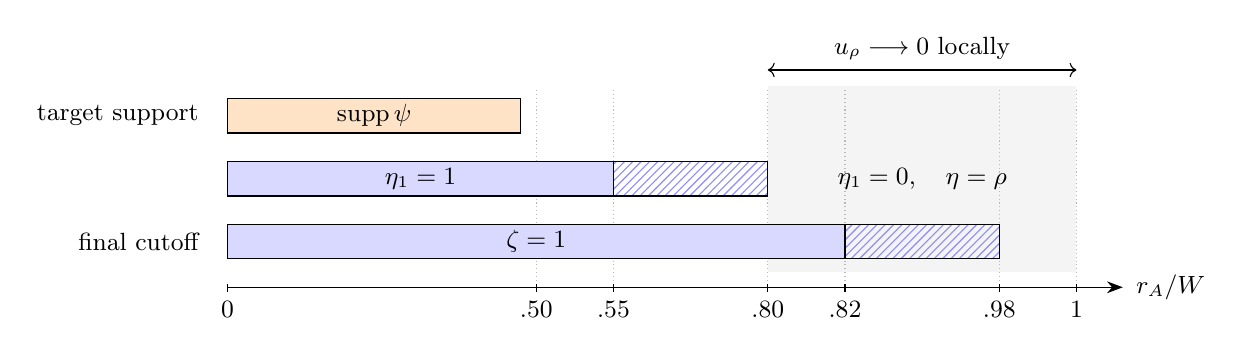
\begin{tikzpicture}[x=.98cm,y=.8cm,font=\small]
 \fill[gray!9] (7,-.4) rectangle (11,2.55);
 \foreach \x in {4,5,7,8,10,11}
   \draw[gray!55,densely dotted] (\x,-.55)--(\x,2.5);
 \fill[orange!22] (0,1.8) rectangle (3.8,2.35);
 \draw (0,1.8) rectangle (3.8,2.35);
 \node at (1.9,2.075) {$\supp\psi$};
 \node[anchor=east] at (-.25,2.075) {target support};
 \fill[blue!15] (0,.8) rectangle (5,1.35);
 \fill[pattern=north east lines,pattern color=blue!45]
                  (5,.8) rectangle (7,1.35);
 \draw (0,.8) rectangle (7,1.35);
 \draw (5,.8)--(5,1.35);
 \node at (2.5,1.075) {$\eta_1=1$};
 \node at (9,1.075) {$\eta_1=0,\quad\eta=\rho$};
 \fill[blue!15] (0,-.2) rectangle (8,.35);
 \fill[pattern=north east lines,pattern color=blue!45]
                  (8,-.2) rectangle (10,.35);
 \draw (0,-.2) rectangle (10,.35);
 \draw (8,-.2)--(8,.35);
 \node at (4,.075) {$\zeta=1$};
 \node[anchor=east] at (-.25,.075) {final cutoff};
 \draw[-{Stealth[length=2mm]}] (0,-.65)--(11.6,-.65);
 \foreach \x/\lab in {0/0,4/.50,5/.55,7/.80,8/.82,10/.98,11/1}
   {\draw (\x,-.60)--(\x,-.72);
    \node[below] at (\x,-.72) {$\lab$};}
 \node[anchor=west] at (11.65,-.65) {$r_A/W$};
 \draw[<->] (7,2.8)--(11,2.8);
 \node[above] at (9,2.8) {$u_\rho\longrightarrow0$ locally};
\end{tikzpicture}
\caption{The spatial cutoffs, with $\eta=\rho+(1-\rho)\eta_1^2$.
The first bar shows the containment $\supp\psi\subset\{r_A<W/2\}$;
hatching indicates where a cutoff may vary.  The graph heights $u_\rho$
constructed below tend to zero in $C^3$ locally outside
$\{r_A\le.8W\}$ as $\rho\downarrow0$, leaving room for the final metric
and drift cutoff.  Spacing is schematic; endpoints are exact multiples of $W$.}
\label{stretch:figure}
\end{figure}

\subsection{Solving the graph equation and obtaining locality}
\label{stretch:equation}

Work for the moment on a closed auxiliary manifold extending a
neighborhood of $\{r_A\le1.1W\}$.  If $M$ is compact, use $M$ itself.
Otherwise, enclose this compact neighborhood in a relatively compact
smooth domain, modify the data to product form near its boundary, and
double.  Extend $h,t$ smoothly and the compactly supported cutoffs by
zero.  Define $\eta$ from the extended $\eta_1$ as above.  This auxiliary
manifold is fixed as $\rho$ tends to zero; all geometric constants in this
subsection may depend on it.

For $0\le\lambda\le1$, consider the equation
\begin{equation}\label{stretch:pde}
 \begin{gathered}
 \diver_{h,t}\mathcal A(\dd u)
     =j(s)F\left(\frac{u-\lambda\psi}{\eta},t\right),\\
 \mathcal A(\dd u)=\frac{\sqrt\mu}{\sqrt{1+s^2}}\nabla_hu,
 \qquad j(s)=\sqrt{\theta+a^2s_0^2},
 \qquad s=|\dd u|_h.
 \end{gathered}
\end{equation}
We solve it within the open domain
$|u-\lambda\psi|/\eta<S_0$.  Both $\mathcal A$ and $j$ are smooth
functions of the covector $\dd u$, including at zero.  The flux derivative
has tangential and radial eigenvalues $k_1/s$ and $(k_1)_s$, respectively;
both are positive for $s>0$ and tend to $a$ at zero.

We first obtain estimates for every smooth solution in this domain.
There is $S_1<S_0$, independent of $\rho,\lambda$, such that
\begin{equation}\label{stretch:height}
 |u-\lambda\psi|\le S_1\eta.
\end{equation}
To see this, compare with $\lambda\psi\pm S\eta$ for $S<S_0$.
Their first two derivatives are uniformly bounded as $S\uparrow S_0$,
whereas $j\ge as_0$ and the poles of $F$ are uniform on the compact range
of $t$.  For $S$ sufficiently close to $S_0$, these functions are strict
upper and lower barriers.  At a positive maximum of a violation, the
gradients agree, ellipticity orders the second derivatives, and $F_x>0$
orders the right sides, a contradiction.  The same fixed $S$ therefore
works for all $\rho,\lambda$.

There is also a gradient bound independent of $\rho,\lambda$.  At a point
of maximum slope, there is nothing to prove if $s<1$.  Otherwise $\mu=1$
in a neighborhood, and \eqref{stretch:pde} is the ordinary graph equation
of Lemma~\ref{pre:angle}, with
\[
 p(x,z,\omega)=\sqrt{1-\omega^2+a^2s_0^2}\,
 F\left(\frac{z-\lambda\psi(x)}{\eta(x)},t(x)\right),
 \qquad \omega=(1+s^2)^{-1/2}.
\]
By \eqref{stretch:height}, the values of $F,F_t,F_x$ range in a compact
set uniformly in $\rho,\lambda$.  Holding $\omega$ fixed and writing
$\xi=(u-\lambda\psi)/\eta$, we have on the graph
\[
 \partial_\nu\left(\frac{z-\lambda\psi}{\eta}\right)
 =\frac{\nu_z-\lambda\,\dd\psi(\nu_h)
                         -\xi\,\dd\eta(\nu_h)}{\eta}.
\]
Thus the zeroth order coefficient of the angle operator is bounded below
by $-C/\eta$, after discarding the nonnegative term $|\mathrm{II}|^2$.
Here $C$ is independent of $\rho,\lambda$.  On the other hand,
\[
 p_z=\frac{jF_x}{\eta}\ge\frac{A_0T}{\sqrt2\,\eta}
\]
at the point under consideration.  At this minimum of $\omega$, the
angle equation gives
\[
 -p_z=\mathcal L\omega\ge-\frac{C}{\eta}\omega.
\]
It follows that $\omega$ is uniformly bounded below, as required.

For each fixed $\rho>0$, these estimates confine the solutions to compact
jet ranges strictly inside the domain of the equation.  The elliptic
estimates described in Section~\ref{pre:elliptic-tools} give all higher
bounds.  The linearization of the left side minus the right side has
zeroth order coefficient $-jF_x/\eta<0$, so it is invertible on the closed
manifold by the maximum principle and linear elliptic theory.  The method
of continuity therefore applies from the solution $u=0$ at $\lambda=0$
to $\lambda=1$.  Write $u_\rho$ for the resulting smooth solution.
The higher estimates used for this continuation may depend on $\rho$;
the height and gradient estimates do not.

The graph equation has now produced a height close to $\psi$.  Its next
property is what permits a compactly supported change of metric:
\begin{equation}\label{stretch:locality}
 u_\rho\longrightarrow0\quad\text{in }C^3
 \text{ on compact subsets of any open region where }
                       \psi=\eta_1=0.
\end{equation}
In such a region $\eta=\rho$.  Expanding \eqref{stretch:pde} in a
coordinate chart gives
\begin{equation}\label{stretch:reaction}
 a^{ij}\partial_i\partial_j u_\rho+b^i\partial_i u_\rho
                         -\frac{c_\rho}{\rho}u_\rho=0,
 \qquad
 c_\rho=j\int_0^1F_x(qu_\rho/\rho,t)\,\dd q.
\end{equation}
The previously established gradient bound makes $(a^{ij})$ uniformly
elliptic and bounded and makes $b^i$ bounded.  The first order terms have
this form because the flux vanishes at zero covector.  By
\eqref{stretch:height} and Proposition~\ref{pressure:law}, $c_\rho$ is
bounded above and below by positive constants, independently of $\rho$.

On a coordinate box with closure in this region, let $\ell_f$ be the
inward affine distance from its face $f$.  For sufficiently small fixed
$\gamma>0$, the function
\[
 C\sum_f\exp(-\gamma\ell_f/\sqrt\rho)
\]
is a supersolution of the operator in \eqref{stretch:reaction}, for all
small $\rho$.  Indeed, its second derivative terms are bounded by a
constant times $\gamma^2/\rho$, its first derivative terms by a constant
times $\gamma/\sqrt\rho$, and its negative zeroth order term dominates
both.  Choose $C$ to dominate the uniform height bound on the faces and
compare with $u_\rho$ and $-u_\rho$.  This proves exponential decay of
the height on every interior subbox.

To turn this into derivative decay, rescale around an interior point by
$x=x_0+\rho y$ and $u_\rho(x)=\rho v(y)$.  The equation takes the
divergence form
\[
 \partial_{y_i}\mathfrak A^i(x_0+\rho y,Dv)
           =\rho\,\mathfrak B(x_0+\rho y,v,Dv).
\]
Here $|v|\le S_1$ by \eqref{stretch:height}, while $Dv=Du_\rho$ is
uniformly bounded.  All coefficient derivatives on these ranges are
uniformly bounded, and ellipticity is uniform.  The interior estimates
from Section~\ref{pre:elliptic-tools} give bounded derivatives of $v$
of every order on smaller fixed balls.  Returning to the original
coordinates yields bounds $C_j\rho^{1-j}$ for derivatives of order $j$.
For fixed nested subboxes $K\subset\operatorname{int}K'$, interior
interpolation gives
\[
 \|u_\rho\|_{C^3(K)}
 \le C\|u_\rho\|_{C^0(K')}^{1/4}
          \|u_\rho\|_{C^4(K')}^{3/4}
       +C\|u_\rho\|_{C^0(K')}.
\]
The $C^4$ norm is at most $C\rho^{-3}$, while the $C^0$ norm decays
exponentially in $1/\sqrt\rho$.  The right side tends to zero, proving
\eqref{stretch:locality}.

\subsection{Curvature balance}
\label{stretch:curvature}

For the slope functions \eqref{stretch:slope-functions},
\[
 0\le-s\beta_s\le2.
\]
Indeed, $-s\beta_s=s\theta_s/[2(1-\theta)]$; on the switching interval
use $s\le.05$ and $\sigma'\le60$, and outside it the formula is immediate.
Thus Lemma~\ref{pre:graph-comparison} applies to $u=u_\rho$.  Denote its
output by
\begin{equation}\label{stretch:raw-data}
 h_u=h+\frac{\theta}{(1-\theta)s^2}\,\dd u^2,
                 \qquad t_u=t-\beta.
\end{equation}
Here $\dd u^2$ denotes $\dd u\otimes\dd u$.
These expressions are smooth across $s=0$: the coefficient of $\dd u^2$
extends as $\mu/[1+(1-\mu)s^2]$.  All comparisons with $h_0$ below take
place in the original neighborhood of $A$; no extension of $h_0$ is
needed.

On $\{s>0\}$, put $e=\nabla_hu/s$ and $b=\sqrt{h_0(e,e)}\le1$.
The rank-one inverse metric formula gives
\begin{equation}\label{stretch:trace}
 \tr_hh_0-\tr_{h_u}h_0=\theta b^2.
\end{equation}
Use $J,H,K,M_1$ as in Lemma~\ref{pre:graph-comparison}: $J$ is the
second fundamental form of the levels of $u$, $H=\tr J$,
$K=-e\log k_1$, and $M_1=H-et-K$.  In particular,
\[
 \Dcal(h_u,t_u)-\Dcal(h,t)\ge\theta E,\qquad
 E=|J|^2+M_1^2+K^2/l^2-2M_1K+2eM_1.
\]
Increasing the drift by $-\beta$ has a controlled effect on the reserve:
\begin{equation}\label{stretch:reserve-increment}
 \frac{(V(t-\beta)-V(t))_+}{\theta}
       \le4(1+s)N(t),\qquad s>0.
\end{equation}
Indeed, if $b_*=-\beta\ge0$, the numerator is at most
$2N(t)b_*+b_*^2$.  When $\theta\le1/2$ one has $b_*\le\theta$.
When $\theta>1/2$, one has $s>1$ and
$b_*\le\tfrac12\log(1+s^2)\le\sqrt s$; these inequalities give
\eqref{stretch:reserve-increment}.

Together with \eqref{stretch:trace}, this identifies the estimate needed
at slopes $s\ge s_0$: it suffices to prove
$E\ge4(1+s)N(t)-\delta b^2V(t_u)$.  Below $s_0$, we will instead use
the adjustable small error in Lemma~\ref{stretch:local}.

To express the graph equation in the normal variables, put, for $s>0$,
\begin{equation}\label{stretch:chi}
 \chi=\frac{j}{k_1}=\sqrt{1+\frac{a^2s_0^2}{\theta}},\qquad
 m_1=\frac{\dd\log\chi}{\dd\log k_1}
       =-\frac{a^2s_0^2}{\theta+a^2s_0^2}.
\end{equation}
The factor $\chi$ normalizes the pressure after division by $k_1$, and
$m_1$ records its derivative.  Directly from these formulas,
\begin{equation}\label{stretch:slope-bounds}
 \begin{gathered}
 -1\le m_1\le0,\qquad 1\le\chi\le2\quad(s\ge s_0),\\
 m_1\le-\tfrac12,\qquad \chi\ge s_0/s,\qquad
 \theta\chi^2\le2a^2s_0^2\quad(0<s\le s_0).
 \end{gathered}
\end{equation}
For $s\le s_0$, substitute $\theta=a^2s^2/(1+s^2)$; for $s\ge s_0$,
use $\theta\ge a^2s^2/(1+s^2)$ to bound $\chi$.

Equation~\eqref{stretch:pde} at $\lambda=1$ says
$M_1=\chi F$, with $F$ evaluated at $(\xi,t)$ and
$\xi=(u-\psi)/\eta$.  Since $e\log\chi=-m_1K$ and
$et=H-M_1-K$, differentiation gives
\[
 eM_1=-m_1KM_1+
       \chi\bigl(F_t(H-M_1-K)+F_xe\xi\bigr).
\]
Completing the $H$- and $K$-squares now yields
\begin{equation}\label{stretch:square-estimate}
 \begin{split}
 E&\ge\chi^2\mathcal C+2\chi F_xe\xi,\\
 \mathcal C&=
 [1-l^2(1+m_1)^2]F^2
 -2[1+l^2(1+m_1)]FF_t-nF_t^2.
 \end{split}
\end{equation}
For clarity, the discarded quantity is exactly
\[
 |J|^2-\frac{H^2}{n-1}
 +\frac{(H+(n-1)\chi F_t)^2}{n-1}
 +\left(\frac K l-l\chi((1+m_1)F+F_t)\right)^2
 +\theta\chi^2F_t^2,
\]
which is nonnegative.  The choice of $j$ now has two useful effects.
At small slope, $m_1\le-1/2$ leaves the coefficient of $F^2$ at least
$3/4$, while $\theta\chi^2=O(a^2)$ makes its eventual error small.
At larger slope, the two alternatives in the pressure law supply the
balance: a large value of $F_x$ is accompanied by a favorable term
$-FF_t$.

\paragraph{Slopes at least $s_0$.}
The pressure bounds imply $F_t^2\le\epsilon|FF_t|$.  Since
$n\epsilon\le1/8$ and $0\le1+m_1\le1$, they give
\begin{equation}\label{stretch:large-C}
 \mathcal C\ge-5\epsilon F_x,\qquad
 -FF_t\ge P_0F_x\ \Longrightarrow\ \mathcal C\ge P_0F_x.
\end{equation}
Indeed, if $FF_t\ge0$, its coefficient has absolute value at most $4$;
if $FF_t<0$, that coefficient contributes at least $2|FF_t|$, whereas
the last term costs at most $n\epsilon|FF_t|$.

If $\eta\ne1$, then $\psi=0$ in a neighborhood, so
\[
 e\xi=\frac{s-\xi e\eta}{\eta}\ge\frac{3s}{4\eta},
\]
using $|\xi|\le S_1<1$, \eqref{stretch:eta-bounds}, and $s\ge s_0$.
Equations~\eqref{stretch:square-estimate}--\eqref{stretch:large-C}
therefore give
$E\ge(3s/2-20\epsilon)F_x\ge sF_x$.
If $\eta=1$, then $\dd\eta=0$ and
$e\xi\ge s-b$ by $|\dd\psi|_{h_0}\le1$.
For $s>8b$ the same estimates give
$E\ge(7s/4-20\epsilon)F_x\ge sF_x$.

It remains to consider $s_0\le s\le8b$ with $\eta=1$.
Here $2\chi(s-b)-s\ge-4$, so $E\ge sF_x-10F_x$.
On the pressure alternative $-FF_t\ge P_0F_x$, the positive term
$\chi^2P_0F_x$ more than pays this loss and gives $E\ge sF_x$.
Otherwise $F_x\le b_0N(t)^2$, and the deficit is at most
$10b_0N(t)^2$.  Since $s\le8$, we have $0\le-\beta<3$, and $T\ge10$
implies
\[
 N(t)^2\le2V(t_u).
\]
This comparison is valid for signed $t$: for $0\le c<3$,
$2V(t+c)-V(t)=(t+2c)^2+T^2-2c^2>0$.
Moreover, $b\ge s_0/8$, and hence
\[
 10b_0N(t)^2\le20b_0V(t_u)
 =\frac{\delta s_0^2}{100}V(t_u)
 \le\delta b^2V(t_u).
\]
We have proved throughout $\{s\ge s_0\}$ that
\begin{equation}\label{stretch:large-slope}
 E\ge sF_x-\delta b^2V(t_u)
   \ge4(1+s)N(t)-\delta b^2V(t_u),
\end{equation}
where the last inequality uses $F_x\ge1000N(t)$ and $s\ge.01$.
Together with \eqref{stretch:reserve-increment} and
\eqref{stretch:trace}, this proves the required curvature inequality
without the small loss $d$ on this slope range.

\paragraph{Slopes below $s_0$.}
Here $1+m_1\le1/2$.  The pressure estimate $|F_t|\le\epsilon|F|$
therefore gives
\[
 \mathcal C\ge(3/4-3\epsilon-n\epsilon^2)F^2\ge F^2/2.
\]
When $\eta=1$, we have $e\xi/\chi\ge-1$.  When $\eta\ne1$ and
$e\xi<0$, we have $s\le|\dd\eta|_h$ and, by
\eqref{stretch:slope-bounds} and \eqref{stretch:eta-bounds},
\[
 \frac{|e\xi|}{\chi}
 \le\frac{|\dd\eta|_h s}{s_0\eta}
 \le\frac{|\dd\eta|_h^2}{s_0\eta}\le C_*.
\]
Using the last bound in Proposition~\ref{pressure:law}, we conclude that
\begin{align*}
 E&\ge\chi^2\bigl[(1/2-2C_*\epsilon)F^2-2C_*b_0V(t)\bigr]\\
  &\ge-C_2\chi^2V(t),\qquad C_2=2C_*b_0.
\end{align*}
The small metric modification now pays for this error.  Namely,
$\theta\chi^2\le2a^2s_0^2$ and
$b_*=-\beta\le\theta\le a^2s_0^2$, so
\[
 (V(t_u)-V(t))_+\le3a^2V(t),
                 \qquad V(t)\le2V(t_u).
\]
Fix $a\in(0,1/2]$ small enough that
\begin{equation}\label{stretch:a-choice}
 (2C_2+3)a^2\le d/4.
\end{equation}
Then the scalar error and the increase in reserve together cost at most
$(d/2)V(t_u)$.  This choice is made before taking $\rho$ small in the
locality argument.

Combining the two slope ranges gives
\begin{equation}\label{stretch:raw-estimate}
 \begin{split}
 \Dcal(h_u,t_u)\ge{}&\Dcal(h,t)+(V(t_u)-V(t))_+\\
 &-\delta(\tr_hh_0-\tr_{h_u}h_0)V(t_u)
                              -(d/2)V(t_u).
 \end{split}
\end{equation}
The inequality extends to boundary points of $\{s>0\}$ by smoothness.
On the interior of $\{s=0\}$ the metric and drift are unchanged, so it
holds there as well.  We have thus retained the full positive increase
of the reserve, apart from the trace loss and half the prescribed small
error.  The remaining half will absorb the final cutoff.

\subsection{Compact support and distance gain}
\label{stretch:finish}

Define the actual output on the original manifold by
\begin{equation}\label{stretch:output}
 h'=h+\zeta(h_u-h),\qquad t'=t+\zeta(t_u-t),
\end{equation}
extending the increments by zero.  The resulting data are smooth and
satisfy $h'\ge h$ and $t'\ge t$; their changes from $h,t$ have compact
support in $\{r_A<W\}$.
On the compact annulus
$\{.81W\le r_A\le.99W\}$, which contains every point where
$0<\zeta<1$, \eqref{stretch:locality} gives $C^3$ convergence
$u_\rho\to0$.  Consequently both the uncut and cut metric and drift
increments tend to zero in $C^2$ there.

To verify the inequality after cutoff without assuming any monotonicity
of $V$, consider its residual
\[
 \begin{split}
 \mathcal R(\widehat h,\widehat t)={}&
 \Dcal(\widehat h,\widehat t)-\Dcal(h,t)
                         -(V(\widehat t)-V(t))_+\\
 &+\delta(\tr_hh_0-\tr_{\widehat h}h_0)V(\widehat t)
                                      +dV(\widehat t).
 \end{split}
\]
By \eqref{stretch:raw-estimate},
$\mathcal R(h_u,t_u)\ge(d/2)V(t_u)\ge dT^2/2$.
The residual is continuous in the indicated $C^2$ data, including the
positive-part term.  Thus
$\mathcal R(h',t')-\mathcal R(h_u,t_u)\to0$ uniformly on the annulus.
For sufficiently small $\rho$, \eqref{stretch:conclusion} follows
there.  Outside this annulus, $\zeta$ is locally constant, with value
one or zero.  The data then agree locally with $h_u,t_u$, where
\eqref{stretch:raw-estimate} applies, or with the original $h,t$.
Completeness follows from $h'\ge h_0$.

It remains to quantify the distance gained.  Use the effective height
$\zeta u_\rho$, extended by zero.  By \eqref{stretch:height} and
\eqref{stretch:cutoffs}, it exceeds $W/5-1$ on $A$ and vanishes on $B$.
Decrease $\rho$ further so that
$|\dd(\zeta u_\rho)|_h\le.01$ throughout the cutoff transition.
Suppose a piecewise smooth curve from $A$ to $B$ had $h'$-length at most
$L_*W$.  Its $h$-length is also at most $L_*W$, and is at least $W$.
The absolute height variation in the cutoff transition, together with
that on $\{\zeta=1,s<.05\}$, is at most $.06L_*W$; repeated visits
are included by integrating the absolute derivative along the curve.
Where $\zeta=0$ there is no height variation.  Thus the remaining
portion, where $\zeta=1$ and $s\ge.05$, carries variation greater than
\[
 (1/5-.06L_*)W-1>.11W.
\]
On that portion $\mu=1$ and $h'=h+\dd u_\rho^2$.  Everywhere else
$h'\ge h$.  Applying the integral triangle inequality to the pair
consisting of the $h$-speed and the absolute height derivative restricted
to this portion gives
\[
 \operatorname{length}_{h'}(\gamma)
 >\sqrt{W^2+(.11W)^2}>L_*W,
\]
a contradiction.  This proves \eqref{stretch:distance-conclusion} and
completes the proof of Lemma~\ref{stretch:local}.

\section{Stretching rounds and the width bound}\label{sec:assembly}
\label{assembly:section}

We now construct the metric and log warps required by
Theorem~\ref{interface:width}.  The local stretching lemma increases
one separation at a time.  Its loss is measured by a decrease in the
trace of a fixed background metric, so a whole family of separations
can be treated without a bound on the overlap of their neighborhoods.
Changing the working scale after each round restores the quadratic
reserve.

\subsection{Summing the local losses}

The following form of the round argument accommodates a drift of
either sign.  It extends the iteration in
\cite[Section~4]{OpenAIWidth} using the positive-part term in
Lemma~\ref{stretch:local}.

\begin{lemma}[One round of separations]\label{assembly:round}
Let $n\ge4$, let
$0<\delta<\min\{1/10,1/(n+1)\}$, and let $W,T$ be supplied by
Lemma~\ref{stretch:local}.  Put $V(t)=t^2+T^2$ and $L_*=1.004$.
Let $h_0$ be a complete smooth metric on a connected smooth
$n$-manifold $M$ without boundary, and let $t_0:M\to\R$ be smooth.
Suppose that, for a real constant $c$,
\[
 \Dcal(h_0,t_0)\ge c+V(t_0).
\]
Let $(A_i,B_i)$ be a finite or countable family of nonempty closed
pairs, with each $A_i$ compact and
$\dist_{h_0}(A_i,B_i)\ge W$.  Suppose there is a locally finite family
of compact sets $K_i$ such that
\[
 \{x:\dist_{h_0}(A_i,x)<W\}\subset K_i\setminus B_i.
\]
Then there are smooth $h_1\ge h_0$ and $t_1\ge t_0$ such that
\begin{align}
 \dist_{h_1}(A_i,B_i)&\ge L_*W\quad\hbox{for every }i,
       \label{assembly:round-distance}\\
 \Dcal(h_1,t_1)&\ge c+\bigl(1-(n+1)\delta\bigr)V(t_1).
       \label{assembly:round-reserve}
\end{align}
The changes are a locally finite sequence of compactly supported
changes inside the sets $K_i$, and $h_1$ is complete.
\end{lemma}

\begin{proof}
Enumerate the pairs and choose $d_i>0$ with $\sum_i d_i<\delta$.
Apply Lemma~\ref{stretch:local} to them successively, keeping $h_0$
as the background metric throughout the round.  The separation
hypothesis is therefore fixed, and increasing the current metric
preserves its domination of $h_0$.  For the current metric and drift
$(H,z)$, define the pointwise functions
\[
 Q=\tr_H h_0,\qquad
 \Lambda=1-\delta(n-Q)-\Sigma,
\]
where $\Sigma$ is the sum of the losses $d_i$ already used.  We claim
that the inequality maintained after every finite number of steps is
\begin{equation}\label{assembly:trace-invariant}
 \Dcal(H,z)\ge c+\Lambda V(z).
\end{equation}
Initially $Q=n$, $\Sigma=0$, and $\Lambda=1$.  At every subsequent
step $0<Q\le n$ and $\Sigma<\delta$, hence
$0<\Lambda\le1$.  Denote the next metric, drift, trace, and coefficient
by $H',z',Q',\Lambda'$, and its small loss by $d$.  Then
$\Lambda'=\Lambda-\delta(Q-Q')-d$.  The local lemma and
\eqref{assembly:trace-invariant} give
\begin{align*}
 \Dcal(H',z')
 &\ge c+\Lambda V(z)+(V(z')-V(z))_+
                 -\bigl(\delta(Q-Q')+d\bigr)V(z')\\
 &\ge c+\Lambda'V(z').
\end{align*}
Here $(a)_+=\max\{a,0\}$, and the second inequality follows from
$a_+\ge\Lambda a$ for $0\le\Lambda\le1$.  This comparison is valid
even when $V(z')<V(z)$.  Since
$\Lambda\ge1-(n+1)\delta$, it proves the asserted reserve at every
finite stage.

Each processed pair attains separation at least $L_*W$, and later
metric enlargements preserve that bound.  The changes are supported
in the locally finite compact family $(K_i)$.  Thus near every point
the metric and drift are unchanged after finitely many steps.  Their
limits $h_1,t_1$ are smooth and satisfy the same local scalar inequality;
metric monotonicity preserves every separation in the limit.
Finally, a smooth metric dominating a complete metric is complete:
an $h_1$-Cauchy sequence converges in $h_0$, and local equivalence of
the two smooth metrics gives convergence in $h_1$.
\end{proof}

\subsection{Proof of Theorem~\ref{thm:main}}

\begin{proof}
\textbf{Initialization.}
Fix $n\ge4$.  Choose $\delta>0$, depending only on $n$, so that
\begin{equation}\label{assembly:delta}
 \delta<\frac1{10},\qquad
 2(n+1)\delta<1-L_*^{-2},\qquad L_*=1.004.
\end{equation}
Take $W,T$ from Lemma~\ref{stretch:local}, and write
$V(t)=t^2+T^2$.  Let $C(n)$ be the constant in
Proposition~\ref{pre:reserve}.  Choose $R_0\ge1$, depending only on $n$,
such that
\begin{equation}\label{assembly:scale}
 \frac{R_0^2}{2}\ge C(n)+T^2,
 \qquad WR_0\ge D_{\mathrm{nat}}(n),
 \qquad D=WR_0.
\end{equation}
These choices precede all metric-dependent constructions.

Let $(M,g)$ satisfy the spectral hypothesis; we may assume $M$ is
nonempty.  Choose a maximal
$D$-separated set of centers $(x_i)_{i\in I}$, and set
\[
 A_i=\overline B_g(x_i,D),\qquad
 B_i=M\setminus B_g(x_i,2D),\qquad
 K_i=\overline B_g(x_i,2D).
\]
The $A_i$ cover $M$, and properness of $g$ makes $(K_i)$ locally finite:
centers whose outer balls meet a compact set lie in a compact
$2D$-neighborhood of that set, which contains only finitely many
$D$-separated points.  Second countability makes $I$ finite or
countable.  If some $B_i$ is empty, then $\diam_gM\le4D$ and a
constant map proves the theorem.  Henceforth every $B_i$ is nonempty.
Choose positive numbers $p_i^*$, including $p_0^*$, with total $1/20$,
and prescribe
\begin{equation}\label{assembly:targets}
 L_i=10+2\pi\sqrt{2/p_i^*}\quad(i\in I).
\end{equation}

By Lemma~\ref{pre:supersolution}, there is a smooth real function $w$
with $\Dcal(g,w)\ge1$.  Dividing a metric by $R^2$ multiplies scalar
curvature, the Laplacian, and squared gradient norms by $R^2$.
Consequently
$\Dcal(g/R_0^2,w)\ge R_0^2$.  Apply Proposition~\ref{pre:reserve} to
$(g/R_0^2,w)$, and multiply its output metric by $R_0^2$.
Call the resulting metric $h^{[0]}$ and its drift $t^{[0]}$.
Then $h^{[0]}\ge g$ is complete and
\begin{align}
 \Dcal(h^{[0]}/R_0^2,t^{[0]})
 &\ge R_0^2+(t^{[0]})^2-C(n)\notag\\
 &\ge \frac{R_0^2}{2}+V(t^{[0]}).
       \label{assembly:initial-reserve}
\end{align}
The original drift $w$ may be unbounded.  The uniform scale in
\eqref{assembly:scale} is available because preprocessing supplies
the quadratic term in the new drift.

\medskip\noindent\textbf{Successive rounds.}

Put $R_j=L_*^jR_0$.  At the start of round $j$ we maintain complete
smooth data $(h^{[j]},t^{[j]})$ satisfying
\begin{equation}\label{assembly:start}
 \Dcal(h^{[j]}/R_j^2,t^{[j]})
       \ge\frac{R_j^2}{2}+V(t^{[j]}).
\end{equation}
A label is called active when
$\dist_{h^{[j]}}(A_i,B_i)\le L_i$; every active label will also satisfy
\begin{equation}\label{assembly:active-distance}
 \dist_{h^{[j]}}(A_i,B_i)\ge WR_j.
\end{equation}
Both assertions hold at $j=0$: the reserve is
\eqref{assembly:initial-reserve}, and $h^{[0]}\ge g$ gives separation
at least $D=WR_0$.

Use the working metric $h_0=h^{[j]}/R_j^2$ for round $j$.
For each active label, its open $h_0$-distance-$W$ neighborhood of
$A_i$ misses $B_i$, by \eqref{assembly:active-distance}.  Therefore
it lies in the fixed original ball $B_g(x_i,2D)\subset K_i$.
Lemma~\ref{assembly:round}, with $c=R_j^2/2$, applies to the active
pairs.  Multiply its output metric by $R_j^2$ to obtain $h^{[j+1]}$,
and denote its output drift by $t^{[j+1]}$.  If there are no active
pairs, keep the metric and drift unchanged.  In either case,
$h^{[j+1]}\ge h^{[j]}$.  Every label still active at the next round
now has separation at least $L_*WR_j=WR_{j+1}$.

The reserve is restored by the new working scale:
\begin{align*}
 \Dcal(h^{[j+1]}/R_{j+1}^2,t^{[j+1]})
 &\ge\frac{R_{j+1}^2}{2}
       +L_*^2\bigl(1-(n+1)\delta\bigr)V(t^{[j+1]})\\
 &\ge\frac{R_{j+1}^2}{2}+V(t^{[j+1]}),
\end{align*}
where \eqref{assembly:delta} makes the coefficient of $V$ greater
than one.  Thus \eqref{assembly:start} holds at every round.  In
original units its constant scalar reserve remains $1/2$.

\medskip\noindent\textbf{The limit and its log warps.}

Each label is active for only finitely many rounds, because its
separation is at least $WR_j$ while active and $R_j\to\infty$.
It remains inactive once its target is exceeded, since all metrics
increase.  Every change associated with label $i$, in every round,
is supported in the same original compact ball $K_i$.  A compact
set meets only finitely many such balls, and each of their labels
is used only finitely many times.  Hence on a neighborhood of any
compact set the metric and drift are unchanged after finitely many
changes in the entire construction.  We obtain smooth data $(h,t)$
with
\begin{equation}\label{assembly:final-drift}
 h\ge g,\qquad \Dcal(h,t)\ge\frac12,
 \qquad \dist_h(A_i,B_i)>L_i\quad(i\in I).
\end{equation}
The metric $h$ is complete by domination of $g$.

It remains to realize the drift by log warps while spending at most
$1/10$ of the scalar reserve.  Dividing a log warp into many equal
parts preserves its sum and reduces the sum of its squared gradients;
see \cite[Section~1.A]{Gromov2024}.  We use the localized construction
of \cite[Theorem~4.3]{OpenAIWidth}, applied to a compactly supported
decomposition of our signed drift.  Take a finite or countable smooth
partition of unity $(\varphi_\nu)_{\nu\ge1}$ with locally finite
compact supports, and put $\tau_\nu=-\varphi_\nu t$.  Then
$\sum_\nu\tau_\nu=-t$.  For each $\nu$, choose an integer $m_\nu\ge1$
so large that
\[
 \frac{1}{m_\nu}\sup_M|\dd\tau_\nu|_h^2
          \le\frac{2^{-\nu}}{10}.
\]
The supremum is finite because $\tau_\nu$ has compact support.
Introduce $m_\nu$ log warps all equal to $\tau_\nu/m_\nu$, and list
all these functions as $(p_\alpha)$.  Repeating each support only
finitely many times preserves local finiteness.  Therefore
\[
 P=\sum_\alpha p_\alpha=-t,
 \qquad
 \sum_\alpha|\dd p_\alpha|_h^2
   =\sum_\nu\frac{|\dd\tau_\nu|_h^2}{m_\nu}\le\frac1{10}.
\]
Substitution into \eqref{interface:scalar} gives
\[
 R(h,(p_\alpha))
 =\Dcal(h,t)-\sum_\alpha|\dd p_\alpha|_h^2
 \ge\frac25.
\]

Equations \eqref{assembly:targets} and \eqref{assembly:final-drift}
now supply all hypotheses of Theorem~\ref{interface:width}.  Its map
has whole fibers of diameter at most $4D+2$ in the original metric
$g$.  Taking
\[
 C_n=4WR_0+2
\]
proves the theorem, since $W$ and $R_0$ depend only on $n$.
\end{proof}

For a quadratic-form lower bound $\lambda>0$, the metric $\lambda g$
has normalized lower bound $1$, since its scalar curvature and
Laplacian are $\lambda^{-1}$ times those of $g$.  Its distances are
$\sqrt\lambda$ times those of $g$, giving the bound
$C_n/\sqrt\lambda$ stated in the introduction.

\bibliographystyle{plain}
\bibliography{references}
\end{document}
